\section{Implementation} \label{sec:implementation_details}

% implementation details
The finite element forward models were implemented in \texttt{C++} and make use of the finite element library \texttt{deal.ii} \cite{dealII93}.

\todo{
All surface and volume integral operators are discretized with Gaussian quadrature using $p_{\text{order}}+1$ one-dimensional (1D) quadrature points in each spatial direction, where $p_{\text{order}}$ is the polynomial order of the finite element space (space)}. 
%$W_h^\porder$.
The experiments in this work are run on a compute blade containing two 32-core AMD EPYC 7543 processors running at 2.80 GHz.

Convergence results are reported using the relative $L^2$-errors 
\begin{equation}
  \erroru(t) = \frac{ \left\lVert \vel(\bm{x}, t) - \velh(\bm{x}, t)\right\rVert_{\LII(\dom_h)} }{ \left\lVert \vel(\bm{x}, t) \right\rVert_{\LII(\dom_h)} }, \qquad 
  \errorp(t) =\frac{ \left\lVert \p(\bm{x}, t) - \ph(\bm{x}, t)\right\rVert_{\LII(\dom_h)} }{ \left\lVert \p(\bm{x}, t) \right\rVert_{\LII(\dom_h)} },
\end{equation}
for vector- and scalar-valued quantities, respectively. Each of the $\LII$-norms over the computational domain $\dom_h$ is calculated using Gaussian quadrature over the element volumes using $p_{\bm{u}} + 3$ for errors in the velocity and $p_{p} + 3$ for errors in the pressure variables.
Unless explicitly specified, the abbreviations $\erroru$ and $\errorp$ refer to the velocity and pressure errors at the final time $T$.

Similarly, unless otherwise specified, all iterative solver tolerances are specified to a relative error of $10^{-12}$ and an absolute error of 

The iterative solvers used in the subsequent test cases use a relative solver tolerance of $10^{-8}$ and an absolute solver tolerance of $10^{-12}$ as tolerance criteria for all system of equations to be solved, unless otherwise specified.

\subsection{Computational considerations}
\label{sec:computational}

HDG methods offer several well-known advantages over standard DG-FEM methods. 
In addition to favorable convergence properties, hybridization of the system by introducing the space \todo{Mph} can lead to a substantial reduction in globally-coupled degrees of freedom as compared to classical DG methods.
However, the complexities associated with the static condensation procedure introduce a set of non-typical computational performance considerations as compared to other high-order methods.
In this section, we provide a brief discussion of practical computational considerations specific to HDG schemes in the context of parallelization and matrix-free solvers. These topics are often overlooked or unaddressed in the literature (to DG/HDG etc ref).

\subsection{Parallelization}%
\label{sec:computational:parallelization}

A commonly cited performance advantage of HDG is the embarrassingly parallel nature of the assembly as well as the local reconstruction of the numerical solution QH UH from the trace quantity UHAT.
Means that people brush this step off computationally, as a parallel implementation should make it trivial.
However there's more to the story than that.

\begin{itemize}
  \item argument: that assembly and reconstruction start to matter at large problem sizes
  \item parallelization needed to beat down assembly and reconstruction time
  \item multi-threaded parallel applications highly dependent on polynomial order
\end{itemize}

though it may seem counter-intuitive, multi-threaded programs can sometimes run slower than their single-threaded or serial counterparts due to several reasons:

Overhead: Threads require resources for creation, termination, and synchronization. The overhead of managing multiple threads can slow down the program, especially if the computation performed by each thread is not significant compared to this overhead.
Contention: When multiple threads try to access a shared resource simultaneously, contention can occur. This could lead to a situation called a lock, where one thread has to wait for another to release a resource. In extreme cases, this can lead to a slowdown known as lock contention, where the threads spend more time waiting to access the resource than doing useful work.
False sharing: Even if different threads are working on different data, if that data is close enough in memory (i.e., in the same cache line), then the hardware can treat it as if it were shared. When one thread updates its data, the hardware will think the entire cache line has been modified and will have to update it across all the cores, leading to a significant slowdown. This is known as false sharing.
Load imbalance: If the work is not evenly distributed across threads, some threads may finish their work early and sit idle, while others are still working. This is known as load imbalance. It can result in the execution time of the program being dominated by the slowest thread.
Non-parallelizable tasks: Some tasks simply can't be parallelized effectively due to their nature, they are inherently serial (or "sequential"). This principle is encapsulated by Amdahl's Law, which states that the maximum improvement to a system's performance is limited by the portion of the system that can't be parallelized.
Memory limits: Every thread created uses some memory for its stack. If the number of threads is too high, it can cause significant memory usage, potentially leading to swapping if the system runs out of physical memory, which can drastically decrease performance.
It's worth noting that developing an efficient multi-threaded program requires careful design to minimize these issues. This can involve techniques such as fine-tuning the number of threads, avoiding contention and false sharing, balancing the load properly, and choosing appropriate data structures and synchronization primitives. But even with all these considerations, there's no guarantee that a multi-threaded solution will always outperform a well-optimized single-threaded one. It highly depends on the nature of the problem and the specific hardware the software is running on.

In this case the synchronization work necessary to ensure no race condition while copying elemental contributions into the global linear system is highly sensitive to problem dimension and polynomial order.
The necessary work on the cell 

In the following, we discretize the problem at different polynomial orders such that the global number of primal degrees of freedom are held constant.
We evaluate the assembly times using both serial and parallelized assembly.
\begin{figure}[htpb]
  \centering
  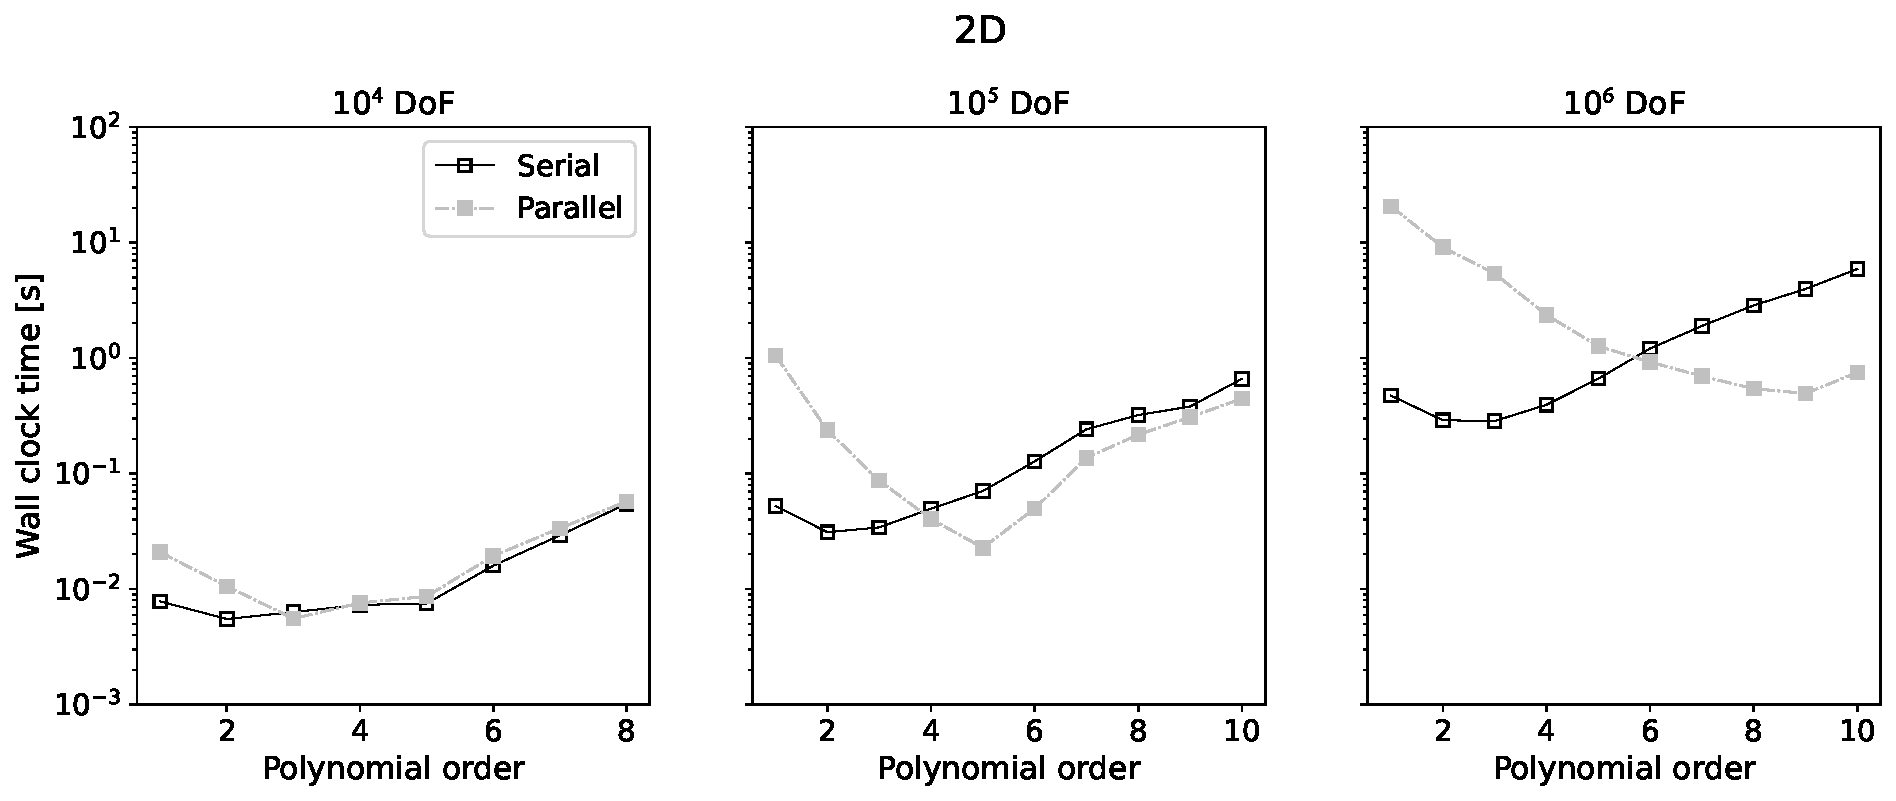
\includegraphics[width=0.8\linewidth]{img/assembly_benchmarking_2D.pdf}
  \caption{Wall clock times for 2D HDG assembly at constant problem size, serial vs. parallel}
  \label{fig:assembly_benchmarking_2D}
\end{figure}

\begin{itemize}
  \item need to give the computer enough work (i.e., large enough problem size)
\end{itemize}

\begin{figure}[htpb]
  \centering
  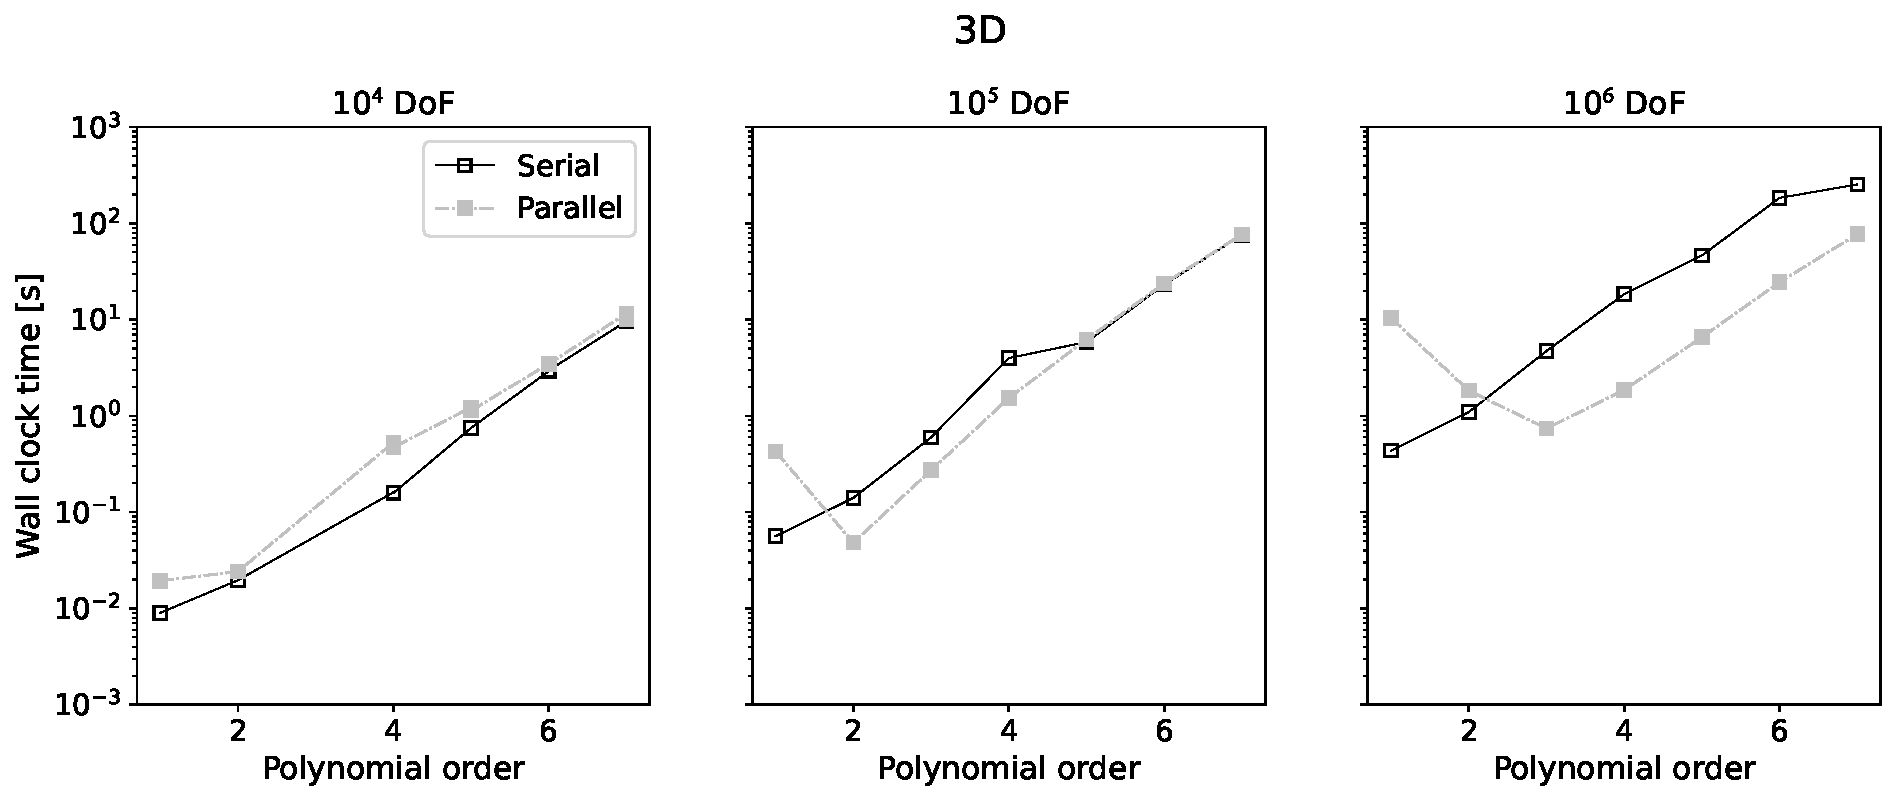
\includegraphics[width=0.8\linewidth]{img/assembly_benchmarking_3D.pdf}
  \caption{Wall clock times for 3D HDG assembly at constant problem sizes, serial vs. parallel}
  \label{fig:assembly_benchmarking_3D}
\end{figure}


It turns out that for one-dimensional problems using any polynomial order less than or equal to $p=10$, it is far more efficient to perform assembly in serial as opposed to in parallel using multi-threading.
This is because the problem dimension leads to element-local systems small enough that the synchronization work between the threads to prevent a race condition copying into the global linear system is much larger than the actual work on the cell.


\subsection{Matrix-free solvers}%
\label{sec:numerical_expeiments:matrix_free}


\subsection{On the solution of the pure Neumann problem}

In the case of pure Dirichlet boundaries on the velocity predictor, the pressure level is undefined. 
To see this, note that if the scalar field $\delta p_h$ is a solution of (\ref{eq:PC_presure_poisson}) with $\Gamma_N = \partial \Omega$, then $\delta p_h + c$ for any $c \in \reals$ is also a solution. 
Discretely, the null space of the linear system arising due to the discretization of (\ref{eq:PC_presure_poisson}) is spanned by the set of constant vectors, implying a singular linear system.

Although crucial to the performance of pressure correction schemes, the issue of finding a solution to the rank-one deficient singular system in such cases receives little attention in the literature, outside of specialized literature for iterative solvers \cite{axelsson_iterative_1996,iankov_finite_2013}.

In \cite{bochev_finite_2005}, the authors rigorously describe strategies for addressing the singular system in a continuous finite element context. 
Here, we extend that discussion to the DG-FEM setting and illustrate computational trade-offs associated with different candidate approaches.

\todo{
This is complicated by the fact that some numerical linear algebra software varies widely in terms of implementation; while some libraries will not solve a singular system (numpy), other direct procedures will do so when they can identify a zero-pivot. 
Similar for iterative solvers.}

\textbf{section TD}
\begin{itemize}[itemsep=1pt]
  \item lit review
  \item three approaches
  \item manufactured solution
\end{itemize}

\subsubsection{Proposed solutions}%

\textbf{Subspace projection.} As a first approach, we apply a subspace projection using a Krylov-solver \cite{vorst_iterative_2003}, making use of the fact that iterative solvers solve singular systems provided that the right-hand side is in the orthogonal complement of the null-space.
\todo{
This modification is ok because we're only removing the null space contribution to the linear system
}

\textbf{Penalty method.}
As a second approach, we apply a penalty-based method which can be interpreted as a regularization.
This method, while simple and independent of linear solver type, involves the specification of a hyperparameter $\gamma$.
As a third approach, we impose a mean-value constraint 
\begin{equation}
  \int_{\Omega}^{} \delta p \,d\Omega = 0
  \label{eq:mean_value_zero_condition}
\end{equation}
into the linear system directly, avoiding the saddle point system that arises as a result of applying the constraint as a Lagrange multiplier \cite{bochev_finite_2005}.

\textbf{Point constraint.} An approach favored by many practitioners is to manually specify the value of the candidate solution at a single point by removing an equation from the discrete system and applying a Dirichlet constraint fixing the value of the solution at that point to an arbitrary constant, eliminating the null space and allowing solution of the linear system using a conventional direct solver.
However, in a finite-element context, the function $\delta_p$ is often represented in the Sobolev space $H^1(\Omega)$ or $L^2(\Omega)$, spaces in which point evaluations do not make sense. 
In these cases, imposing such a constraint can render the variational problem ill-posed.
A typical manner of fixing this is to specify the value of the solution along a measurable subset of the domain; typically an element face; while this constraint is well-posed, it's also undesirable, because specifying that the value of the numerical solution along the face will change the character of the numerical solution and thus the physics.

\subsubsection{Computational benchmarks}

In order to investigate the performance of each proposed method to solve the pure Neumann problem, we asses the convergence, accuracy, and efficiency of each method over a wide range of problem sizes and polynomial degrees $p$.
We consider the analytical solution
\begin{equation}
    \deltap^* = \frac{1}{3} \sin\left(-\frac{\pi}{2} x \right) \cos\left(2\pi y\right),
\end{equation}
(Figure \ref{fig:dp_neumann_problem_analytical}, left) with boundary conditions and forcing function deduced from the exact solution over the computational domain $\Omega = [-1, 1]^2$. 
By symmetry, we have that the exact solution $\delta_p^*$ is analytically zero-mean in the sense of equation (\ref{eq:mean_value_zero_condition}).
Additionally, the value of the boundary condition $g_N = \nabla \delta_p^* \cdot\bm{n}$ vanishes algebraically over the boundary $\partial \Omega$, imitating the boundary conditions imposed in the pressure corrector step.
\begin{figure}[htpb]
  \centering
    \begin{subfigure}{0.45\textwidth}
      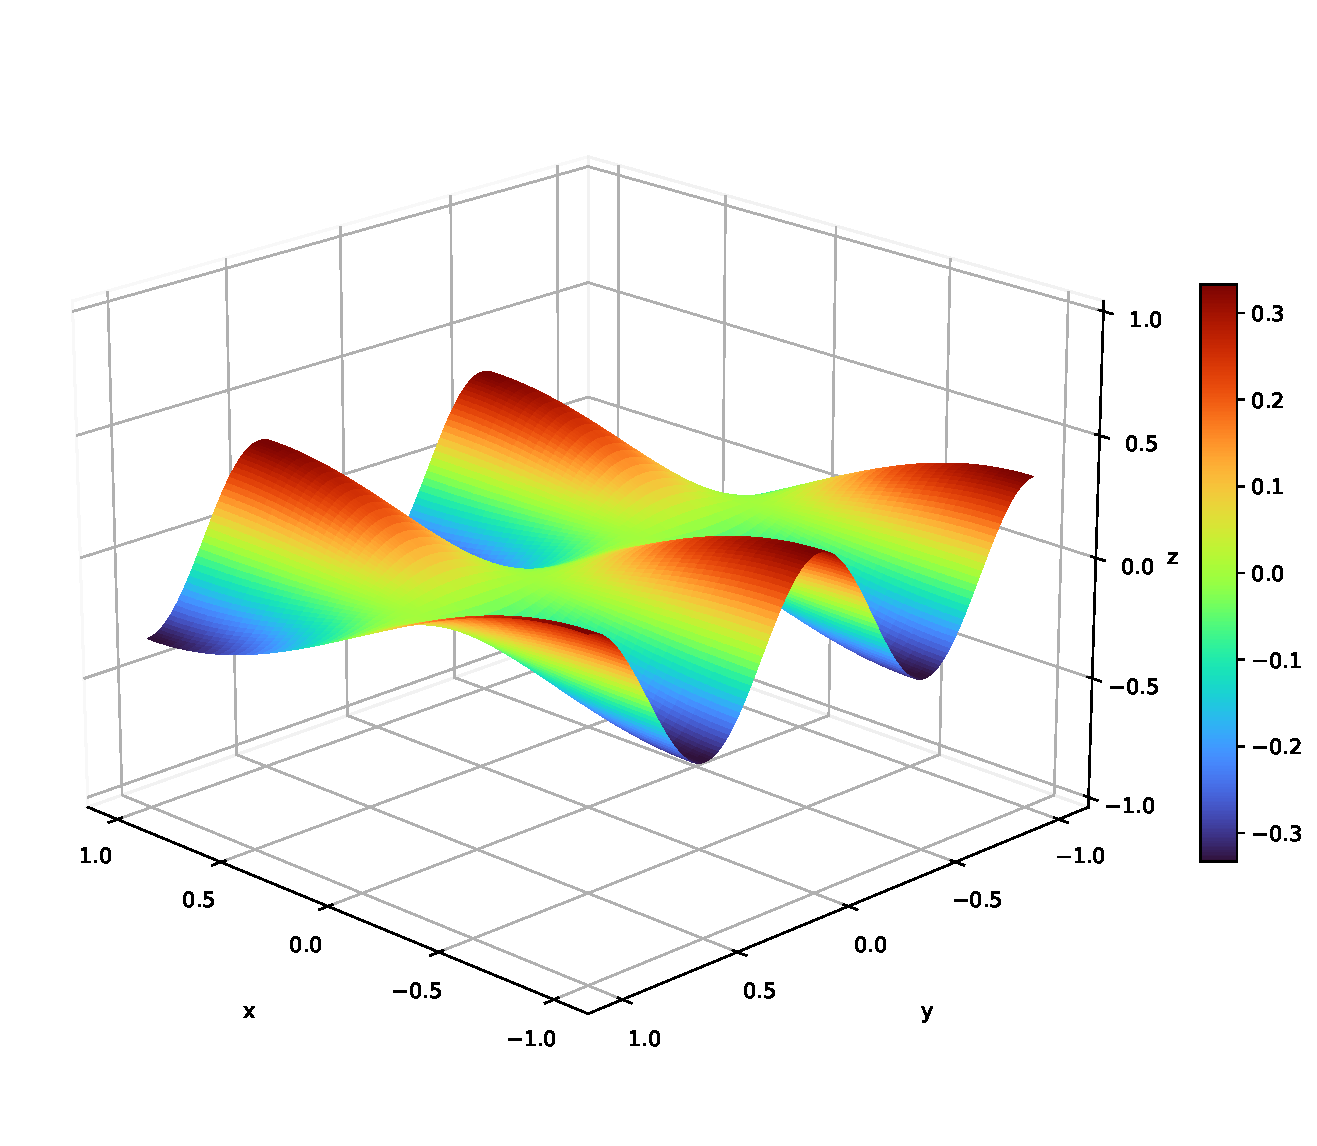
\includegraphics[height=5.75cm]{img/dp_study_analytical.pdf} 
    \end{subfigure}
    \begin{subfigure}{0.45\textwidth}
        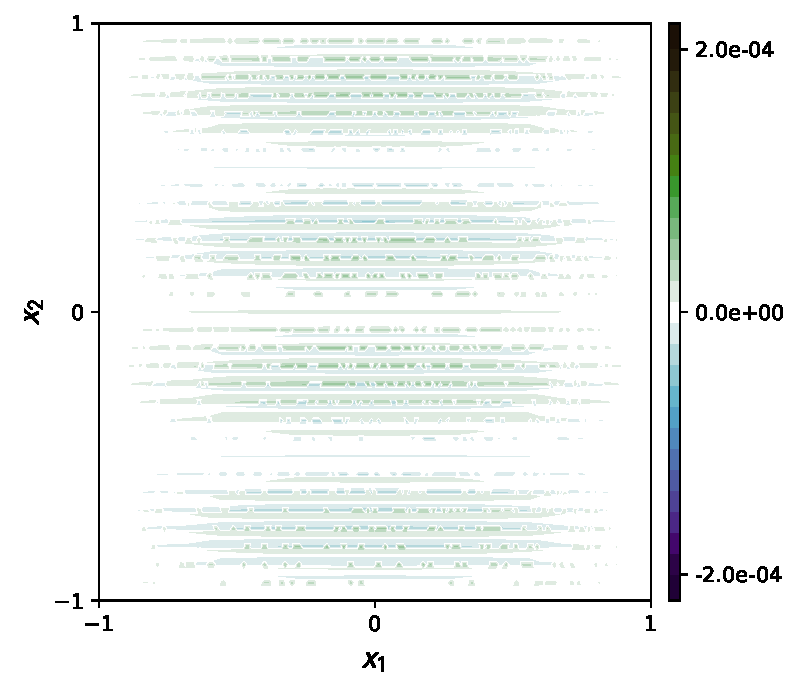
\includegraphics[height=5cm]{img/PNP_32x32_errors.pdf}
    \end{subfigure}
      \caption{(Left) Analytical solution of the pure Neumann problem. 
        (Right) Distribution of numerical errors in the gradient $\nabla\delta_p^* - \qdph$ over the computational domain for a mesh of $32\times 32$ elements at polynomial order $p=3$.}
  \label{fig:dp_neumann_problem_analytical}
\end{figure}
We consider a uniform Cartesian grid consisting of quadrilateral elements of length $L/2^{\ell}$ in each spatial dimension, where the integer $\ell = 0, 1, \ldots$ denotes the level of refinement.
To assess the convergence of the primal unknown $\deltap$, the integral mean level of the numerical solution is subtracted as post-processing to agree with the analytical solution.
All iterative solves are performed using conjugate gradient (CG) iterations to solve for the trace unknowns $\hat{\delta}_{p,h}$, from which the primal solution $\dph$ and its gradient $\bm{q}_{\deltap,h}$ are reconstructed.

All three methods achieve optimal $p+1$ order convergence to the exact solution in both the primal $\dph$ and gradient $\qdph$ unknowns, respectively, before the iterative solver tolerance and finite-precision effects begin to pollute the convergence order. 
Figure \ref{fig:INS:convergence_singular_system_projection} illustrates the convergence history of the primal unknown $\dph$ for the projection approach, both from the perspective of mesh resolution and in globally-coupled trace unknowns.
The errors and orders of convergence in the $\LII$-norm are presented in tabular form in \ref{sec:convergence_history_pure_neumann}.
In what follows, we demonstrate the subspace projection approach to be the computationally superior method; therefore, we present the convergence results for the projection method and omit the others for brevity. 

An examination of the spatial distribution of the errors in the numerical gradient\footnote{%
We compute the directional error $\nabla \delta_p^* - \qdph$ over each element and plot the $x_1$-component. The results are similar for the gradient in the $x_2$ direction. We consider the gradient rather than the primal variable, because the gradient is the quantity that is used in the projection method detailed in \S\ref{sec:temporal_discretization}.
}%
over the computational domain (Figure \ref{fig:dp_neumann_problem_analytical}, right) illustrates that they are neither disproportionately large on the domain boundary, nor are they localized around a single point, problems that have been known to plague the penalization and point constraint methods, which depend on a specific choice of degree of freedom for their implementation \cite{bochev_finite_2005,guermond_overview_2006}.

\begin{figure}[ht]
    \centering
    \begin{subfigure}{0.45\textwidth}
        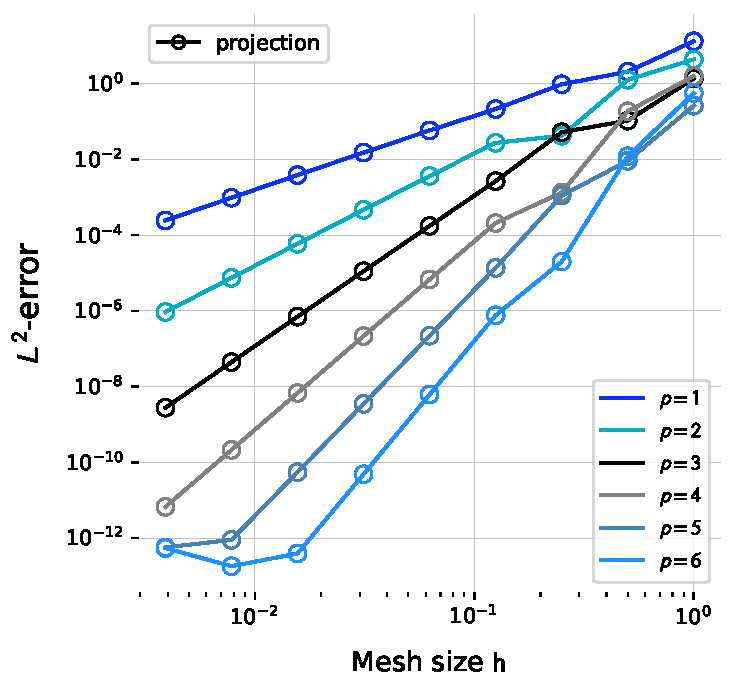
\includegraphics[height=7cm]{img/PNP_conv_2D.pdf}
    \end{subfigure}
    \begin{subfigure}{0.45\textwidth}
        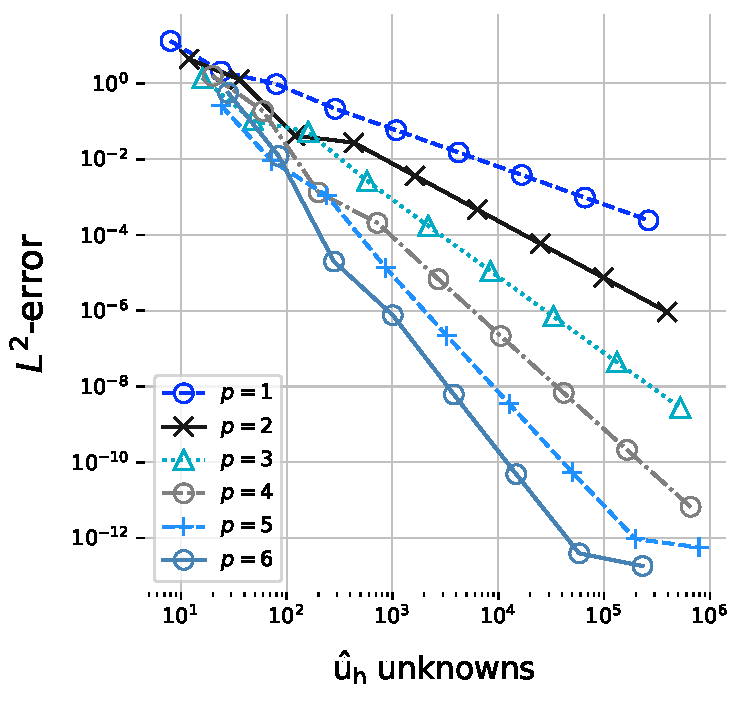
\includegraphics[height=7cm]{img/PNP_conv_2D_dofs.pdf}
    \end{subfigure}
    \caption{Errors in the primal unknown $\left\lVert \delta_p^* - \dph \right\rVert_{\LII(\dom)} $ for the singular Neumann problem (2D) treated with subspace projection. Convergence is shown with respect to mesh size as well as number of globally-coupled unknowns. Optimal convergence is achieved for all polynomial orders.
    Convergence history data is tabulated in \ref{sec:convergence_history_pure_neumann}}
    \label{fig:INS:convergence_singular_system_projection}
\end{figure}

Given the comparable order of convergence to the analytical solution for all three approaches, we compare their relative computational advantages. 
Reporting a condition number for the resultant linear system solved with each method is not feasible. 
On one hand, the problem sizes reported in this work are large enough to make direct computation of the eigenvalue spectrum intractable.
Moreover, as the subspace projection transformation is applied at each conjugate gradient iteration, there is not a single resultant linear system for which to compute a condition number.
Therefore, as a practical indication of the conditioning of each algorithm, we examine the efficiency of the iterative solver.
Figure \ref{fig:PNP_treatments_CG_iterations} shows the number of conjugate gradient iterations required to achieve convergence to the specified solver tolerance (without preconditioning) over a wide range of problem sizes.
We observe that the point constraint and penalization methods require many more iterations to converge than the subspace projection approach across polynomial orders, typically between a factor of two and a factor of ten.
Since the subspace projection requires removal of the mean at every conjugate gradient iteration and the other two methods do not, we also benchmark the performance of each algorithm in terms of the overall $\LII$-error in the primal solution variable as a function of the wall clock time to solution of the linear system for the trace unknown $\hat{\delta_p}_h$ in Figure \ref{fig:PNP_treatments_wall_time}.
We observe that the subspace projection approach equals or outperforms the other two methods over a wide range of problem sizes, with the advantage increasing as a function of polynomial order.

\begin{figure}[ht]
    \centering
    \begin{subfigure}{0.45\textwidth}
        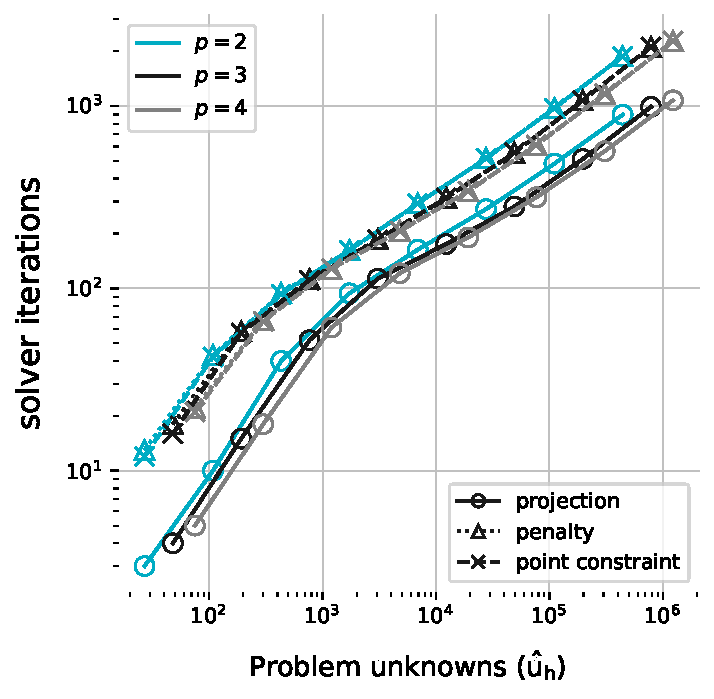
\includegraphics[height=7cm]{img/PNP_solver_iterations.pdf}
        \caption{}
        \label{fig:PNP_treatments_CG_iterations}
    \end{subfigure}
    \begin{subfigure}{0.45\textwidth}
        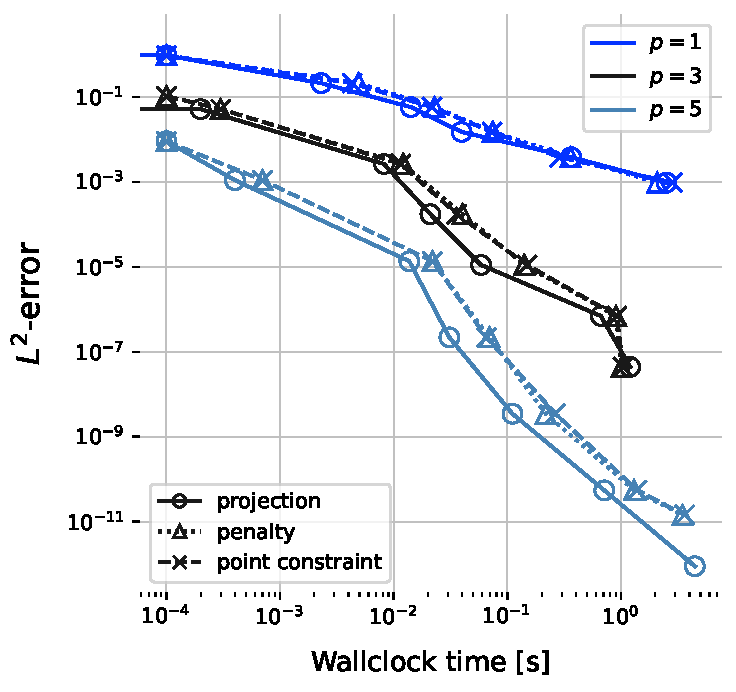
\includegraphics[height=7cm]{img/PNP_treatment_wall_times.pdf}
        \caption{}
        \label{fig:PNP_treatments_wall_time}
    \end{subfigure}
    \caption{Performance comparisons of the different singularity treatments.
    (Left) Number of conjugate gradient iterations required for convergence for each method at different problem sizes and polynomial orders.
    (Right) $\LII$-error achieved in the primal unknown $\dph$ as a function of wall clock time-to-solution of the global linear system for the trace unknown, shown at different problem sizes spanning from $10^1$ to $10^6$ trace degrees of freedom, and different polynomial orders.}
    \label{fig:PNP_treatment_performance}
\end{figure}

In conclusion, we have found the subspace projection approach to be a stable, robust, and accurate method for numerically solving the singular system arising from the discretization of the pure Neumann problem occurring in the case of pure Dirichlet boundary conditions on the velocity.
Furthermore, we have demonstrated it to be a superior method computationally, delivering better accuracy with a shorter time-to-solution than both the point-constraint and penalization approaches, and without the need to calibrate any additional hyperparamters or to single out a particular problem degree of freedom for the imposition of a constraint.

\section{Numerical experiments} \label{sec:numerical_experiments}

\subsection{Verification}

\subsubsection{Kovasnay flow}%
\label{ssub:kovasnay_flow}


Following \cite{hesthaven_nodal_2008}, to provide verification of the nonlinear, pressure, and viscous spatial derivatives independent of the temporal discretization, we test the method using the Kovasnay analytical solution to the Navier--Stokes equations.

\begin{equation}
  \begin{aligned}
    \bm{u(\bm{x})} &= 
    \begin{pmatrix}
      1 - e^{\lambda x} \cos(2 \pi y) \\
      \frac{\lambda}{2\pi} e^{\lambda x} \sin(2\pi y)
    \end{pmatrix}, \qquad
    p(\bm{x}) = \frac{1}{2} \left(1 - e^{2\lambda x}\right),
  \end{aligned}
  \label{eq:kovasnay_flow}
\end{equation}
where the parameter 
\begin{equation}
\lambda = \frac{1}{2\nu} - \sqrt{\frac{1}{4\nu^2} + 4\pi^2}.
\end{equation}

We consider a domain $\Omega = [-0.5,1]\times [-0.5, 1.5]$ with the domain boundary consisting of inflow and outflow segments $\bnd = \bndIn\cup \bndOut$ with $\bndOut = \left\{\bm{x}\mid x_1 = 1\right\}$. 
For the velocity field, Dirichlet boundary conditions on the velocity field at the inflow boundary $\bndIn$ and Neumann boundary conditions at the outflow boundary $\bndOut$ are deduced from the exact solution. 
Similarly, the exact solution provides the directional derivative normal to the boundary for the Neumann pressure boundary condition at the inflow boundaries $\bndIn$ and the Dirichlet boundary conditions on the pressure at the outflow. 
These boundary conditions are summarized in Table \ref{tab:Kovasnay_BCs}. \\

\begin{table}[htpb]
  \centering
  \begin{tabular}{ccc}
  \hline
    & $\bndIn = \bnd \setminus \bndOut$ & $\bndOut = \bnd \cap \left\{\bm{x}\colon x_1 = 1\right\}$ \\
  \hline
  $\bm{u}$ & $\bm{g_D} = \bm{u}(\bm{x})$ & $\bm{g_N} = \nabla \bm{u}\cdot\bm{n}$ \\
  $\bm{p}$ & $g_N = \nabla p\cdot\bm{n}$ & $g_D = p(\bm{x})$ \\
  \hline
  \end{tabular}
  \caption{Summary of boundary conditions \S\ref{ssub:kovasnay_flow}.}
  \label{tab:Kovasnay_BCs}
\end{table}

The simulation is performed for one time integration step with viscosity parameter $\nu = 1/40$.

\subsection{Vortex flow}
Spatial convergence test, temporal convergence test

\subsection{Unsteady Stokes Flow}

The review paper \cite{guermond_overview_2006} solves the unsteady Stokes problem

\begin{equation}
  \begin{aligned}
    \bm{u}(\bm{x}, t) &= \pi \sin t 
    \begin{pmatrix}
      \sin( 2\pi y) \sin^2( \pi x) \\
      -\sin(2 \pi x) \sin^2(\pi y)
    \end{pmatrix} \\
    p(\bm{x}, t) &= \sin(t)\cos(\pi x) \sin(\pi y)\\
  \end{aligned}
  \label{eq:MS_stokes_guermond}
\end{equation}
where the source term $f= u_t -\nu \nabla \cdot( \nabla \bm{u} ) + \nabla p $.

In \cite{fehn_stability_2017}, we have
\begin{equation}
  \begin{aligned}
  \bm{u}(\bm{x}, t) &= 
  \begin{pmatrix}
    \sin(x) (a\sin(a y) - \cos(a)\sinh(y)) \\
    \cos(x) (\cos(a y) + \cos(a)\cosh(y))
  \end{pmatrix}
  \exp(-\lambda t),\\
    p(\bm{x}, t) &= \lambda \cos(a) \cos(x) \sinh(y) \exp(-\lambda t)
  \end{aligned}
  \label{eq:MS_unsteady_stokes_fehn}
\end{equation}
where $\lambda = \nu(1 + a^2)$ $\nu = 1$ and $a = 2.883356$ on a domain of  $\Omega = [-1, 1]^2$; they take $[0, T] = [0, 0.1]$ and Dirichlet boundary conditions everywhere, $\Gamma = \Gamma_D$.


\subsection{Taylor-Green vortex flow}
Is this the same test case as in Hesthaven?

\subsection{Pipe flow}
\subsection{Backward facing step}
\subsection{Lid-driven cavity flow}
\subsection{Lock Exchange?}
\subsection{Lab RTI flow?}

